% =====================================================================================================
% Experiments (the \section and the label sec:experiments are in main.tex; this file has no \section).
% Sources of the numbers: results/digest.md and results/*_summary.json (validation_book, B3, B2, B1, GammaDelta, A3,
% A2, A4, A4b; all final, A4_summary.json and A4b_summary.json of Nov. 11, 14:35 and 13:55); results/findings.md
% Sections 0--8 for their reading. Derived numbers (ratios of counts, window and local slopes, seed spreads, products of
% measured ratios) are computed from these files; the GD monotonicity exceptions of Section exp-B2 are the keys
% gd_mu_eff_increasing_steps, gd_mu_eff_increase_max_rel and gd_D_max_after_increase of B2_summary.json, and the
% componentwise maxima and sign statistics of Section exp-A3 are in A3_summary.json. Computed from the cached runs: the
% comparison of the product of exact contractions with the realized V_t (results/B3.pkl, seed 0,
% vrlab.analysis.trajectory_bounds), the run lengths of Section exp-B1 (results/B1.pkl), the speed-ups of Section exp-A3
% over passes 2-20 and the lengths of its pooled windows (16 to 60 passes; results/A3.pkl) and the counts of Section
% exp-A2 with stored reference gradients (grad_evals - iters in results/A2.pkl). The exact supremum R_P^2 of Definition
% B1-kappaP, max_i lmax(P^{-1/2}(x_i x_i^T/4 + lam I)P^{-1/2}), is computed on the B1 problems regenerated with data
% seed 0. Values of the book's Figure 5.4 are read from the figure (p. 150); its companion code is the file
% logistic_sgd_saga.m distributed with the book. Seed spreads of the counts
% (max/min - 1 per kappa, maximum over kappa): grads_min/grads_max of A4_summary.json for (H) and (R) (L-Katyusha 6.2%
% and 4.7%), per-seed counts of results/A4b.pkl for (S) and (A) (L-Katyusha 6.4% and 8.4%).
% Figures: each figure environment follows the paragraph that first discusses it and keeps its project figure name
% (0, 1, 2, 3, B2, B1, C, A3, A2, A4b, A4) through a local renewal of \thefigure; the theory notes (Appendices) refer
% to 'Figure B2 of the report', 'Figures 1--3 of the report', 'Figure C of the report', etc.
% =====================================================================================================

\subsection{Common protocol}\label{sec:exp-protocol}

\paragraph{Problems.}
Logistic regression uses the generator of Section~\ref{sec:setting} with $n=1000$, $d=50$, the covariance spectrum
$j^{-\alpha}$, $\alpha\in\{0,1,2\}$ (population condition numbers $1$, $50$ and $2500$), and $\lambda=\frac14/(\kappa-1)$,
so that $\kappa=R^2/\mu$ exactly, with $R^2=\max_iL_i=\frac14+\lambda$ and $\mu=\lambda$. One data set $(x_i,y_i)_{i\le n}$ is
drawn per $\alpha$ (data seed $0$) and shared by all values of $\kappa$, which only set $\lambda$; the seeds reported below
are sampling seeds, and all runs start at $\theta_0=0$ (SAGA
with $z_i^{(0)}=\fip(\theta_0)$). The nominal $\kappa$ is a worst case: over the fifteen problems of
Section~\ref{sec:exp-B3} ($\kappa$ from $10$ to $10^5$), $L_F/\mu$ ranges from $1.2$ to $8.1\cdot10^3$ and
$\lmin(F''(\etastar))/\mu$ from $1.0$ to $70$. The quadratic instances have $n=16$ components: (H)~the block-separable
Nesterov chains of Section~\ref{sec:setting} (normalization of~\cite{lan2018optimal} with Nesterov's chain, $\kappa$ exact,
$L_F=R^2/n$, blocks of length $m=64$ or $256$); (R)~block quadratics with eigenvalues drawn log-uniformly in $[1,\kappa/n]$, random
eigenbases and Gaussian linear terms ($m=256$, one instance per seed); (S)~the instance~\eqref{eq:instance} of
Appendix~\ref{sec:lower_bound} (shared regularizer, $m=256$), whose nominal $\kappa$ exceeds the effective
$\kappa_{\rm eff}=R^2/\lmin(F'')$ of~\eqref{eq:kappaeff} once the chain is exhausted; (A)~the aligned instance of the same
appendix, one chain of length $m=2048$ shared by all components, so that $L_F=R^2$. Minimizers are obtained by direct
solves, and every method receives the exact constants of its instance: $R^2=\max_i\lmax(f_i'')$,
$\mu=\lmin(F'')$ and $L_F=\lmax(F'')$ (on (S) the methods are thus tuned with $\kappa_{\rm eff}$), and for
logistic regression $\mu=\lambda$ and $L_F=\lmax(\hat\Sigma)/4+\lambda$ with $\hat\Sigma=\frac1n\sum_ix_ix_i^\top$.

\paragraph{Exact one-step quantities and precision floors.}
No one-step expectation is estimated by sampling: given the state, $i(t)$ takes $n$ equally likely values, so the
conditional expectations of \resref{lem:B3-identities}, hence the exact conditional contraction
$\rho_{\rm exact}(t)=\E[V_t\mid\mathcal F_{t-1}]/V_{t-1}$ (\resref*{prop:B3-exact}), the tightness ratios
(\resref*{def:B3-ratios}), $\muEff$, $\LEff$ and the
attribution chains (\resref*{prop:B3-attribution}), are computed exactly in $O(nd)$ operations; for L-Katyusha,
$\E[\Psi_{t+1}\mid\text{state}]$ enumerates the $n$ indices and both outcomes of the coin that refreshes the reference
point ($O(n^2d)$). They are evaluated every $n/10$ iterations (every iteration when $n=16$) and checked by the test
suite (Appendix~\ref{app:repro}); they are exact given the visited states, but their products along a trajectory are
realized quantities, not expectations (Section~\ref{sec:B3-traj}). For logistic regression, $\etastar$ comes from a
damped Newton method run to $\norm{\Fp(\etastar)}\le10^{-15}$ or stagnation, so that its squared error is at most
$\norm{\Fp(\etastar)}^2/\mu^2$: at most $2.1\cdot10^{-21}$ on the problems of Section~\ref{sec:exp-B3} whose runs reach
$10^{-18}$ (the runs at $\kappa=10$, $\alpha=1$ indeed stall at $1.3\cdot10^{-21}$), hence a relative error of at most about
$10\%$ on $\norm{\theta_t-\etastar}^2=10^{-18}$, and at most $7\cdot10^{-20}$ at $\kappa=10^5$, $\alpha=0$, whose runs stay
above about $10^{-13}$. Records below the precision of these computations are discarded: SAGA records with
$V_t<10^{-18}$, states with $\norm{\theta_t-\etastar}^2<10^{-18}$ in
Section~\ref{sec:exp-B2}, and L-Katyusha records with $\Psi_t<10^{-10}$ (the $W$-term of $\Psi$ amplifies rounding
errors by $\theta_2(1+\theta_1)/(p\theta_1)\ge250$).

\paragraph{Runs, gradient counts and slopes.}
The steps are $1/(4R^2)$ for SAGA, $1/(6R^2)$ for L-SVRG (Theorem~5 of~\cite{kovalev2020dont}) and $1/L_F$ for gradient
descent (GD) and Nesterov's accelerated gradient (AGD, momentum $(\sqrt{L_F/\mu}-1)/(\sqrt{L_F/\mu}+1)$); L-Katyusha uses
the parameters of Theorem~11 of~\cite{kovalev2020dont}: $\theta_2=\frac12$, $\theta_1=\min\{\sqrt{2n/(3\kappa)},\frac12\}$,
$p=\frac1n$, $\eta=1/(3\theta_1)$, with $\kappa=R^2/\mu$ computed, like the momentum of AGD, from the exact constants of the
instance.
\begin{center}
\small
\begin{tabular}{@{}lp{8.6cm}cp{3.6cm}@{}}
\toprule
Section & problems & seeds & length of the runs \\
\midrule
\ref{sec:exp-validation} & book setting, $d=40$, $n\in\{10^3,10^4\}$ & 1 & 50 passes \\
\ref{sec:exp-B3} & logistic, $\kappa\in\{10,10^2,\dots,10^5\}$, $\alpha\in\{0,1,2\}$ & 5 & 100 passes \\
\ref{sec:exp-constants} & logistic, $\kappa=10^3$, $\alpha=1$, $\gamma R^2\in\{\frac18,\frac14,\frac13,\frac12,1,2,4\}$ & 3 & 40 passes \\
\ref{sec:exp-B2} & logistic, $\kappa\in\{10^2,10^3,10^4\}$, $\alpha\in\{0,1,2\}$ & 1 & 60 passes; GD at most 400 steps \\
\ref{sec:exp-B1} & logistic, $\kappa=10^3$, $\alpha\in\{1,2\}$, four metrics $P$ & 5 & 100 passes \\
\ref{sec:exp-A3} & (H) with $m=64$, $\kappa=10^4$; logistic, $\kappa\in\{10^3,10^4\}$, $\alpha=1$ & 3 & 60 passes \\
\ref{sec:exp-A2} & (H) with $m=64$, $\kappa=10^4$; logistic, $\kappa=10^4$, $\alpha=1$ & 1 & to relative error $10^{-10}$ \\
\ref{sec:exp-A4} & (H), (R): $\kappa\in\{10^2,3\cdot10^2,\dots,10^5\}$, 3 seeds; (S): $\kappa\in\{10^2,3\cdot10^2,\dots,10^6\}$ and (A): $\kappa\in\{10^2,3\cdot10^2,\dots,10^5\}$, 2 seeds & 2--3 & to relative error $10^{-8}$ \\
\bottomrule
\end{tabular}
\end{center}
The SAGA and L-Katyusha runs of Sections~\ref{sec:exp-B3}--\ref{sec:exp-A3} also stop when
$\norm{\theta_t-\etastar}^2\le10^{-26}$ ($\norm{\theta_t-\etastar}_P^2\le10^{-26}$ in Section~\ref{sec:exp-B1}: the runs with the
statistical and Hessian metrics, and with the Jacobi metric for $\alpha=1$, stop after 44 to 72 passes, at
$\norm{\theta_t-\etastar}^2$ between $10^{-24}$ and $3\cdot10^{-23}$, and the curves of Figure~\ref{fig:B1} end with the
shortest run). The budget of Section~\ref{sec:exp-A2} is 200 passes on logistic regression and $9.2\cdot10^4$ passes on
(H). In Section~\ref{sec:exp-A4} a run stops at the first recorded iterate with
$\norm{\theta-\etastar}^2\le10^{-8}\norm{\theta_0-\etastar}^2$, at an iteration cap (above the theoretical count of the
method, or at the level of that of SAGA for the two schemes without a guarantee), at a CPU-time budget, or when it
diverges; capped runs would not enter the fits, but in the final sweeps no run was capped. Iterates are recorded every
$n/20$ iterations in Sections~\ref{sec:exp-B3}, \ref{sec:exp-B2} and~\ref{sec:exp-B1}, every $n/10$ in
Sections~\ref{sec:exp-validation}, \ref{sec:exp-constants}, \ref{sec:exp-A3} and~\ref{sec:exp-A2} (every iteration when
$n=16$) and every $n/4$ in Section~\ref{sec:exp-A4}; GD and AGD are recorded at every iteration. A component gradient
counts $1$ and a full gradient $n$: SAGA pays $n$ initially and $1$ per iteration; L-SVRG, L-Katyusha and the naive
schemes pay $n$ initially, $2$ per iteration ($\fip(x)$ and $\fip(w)$, the latter charged as if recomputed although the
code stores the $n$ gradients at $w$) and $n$ per refresh of the reference point (probability $1/n$), i.e.\ $3$ per
iteration on average, against $2$ with stored reference gradients, the convention of \resref{prop:A4} and of the
other bounds of Appendix~\ref{sec:lower_bound}: their measured counts are thus about $\frac32$ times those of that
convention, which changes constants, not slopes; GD and AGD pay $n$ per iteration. Counts to a target are interpolated
log-linearly between records, except the counts to $10^{-10}$ of Section~\ref{sec:exp-A2}, which are read at the first record below the
target, where the runs stop. Speeds are contraction exponents per pass ($n$ iterations), $-n\log\rho$ for
a factor $\rho$ per iteration (at most about $\frac13$ for the bound of Proposition~\ref{prop:59}), and the
\emph{speed-up} is the ratio of the exact to the certified exponent; empirical exponents are least-squares slopes of
$\log\norm{\theta_t-\etastar}^2$ against $t$ over a window of passes, averaged over seeds. Complexity exponents are
least-squares slopes $b$ of $\log\bar T$ against $\log\kappa$ (or $\log\kappa_{\rm eff}$), where $\bar T$ is the geometric
mean over the seeds of the counts at each $\kappa$, fitted over $\kappa\ge10n$ ($K$ values of $\kappa$) unless stated
otherwise, and reported as $b\pm h$, with $h=t_{0.975,K-2}\,\mathrm{se}(b)$ the half-width of the $95\%$ Student interval
with $K-2$ degrees of freedom. The seeds are independent replicates for the stochastic methods, whereas GD and AGD are
deterministic on (H), (S) and (A) (on (R) each seed draws its own instance). Fitting the per-$\kappa$ means treats every
method alike, and the interval then measures the scatter of these means about a single power law over the fitted range,
essentially the departure of the curve from a power law: the seed-to-seed spread of the counts is small ($\max/\min-1$ at
most $3\%$ for SAGA, L-SVRG, and GD and AGD on (R), $6.4\%$ for L-Katyusha on (H), (R) and (S) and $8.4\%$ on (A), and
$26$--$30\%$ for the naive scheme, whose setting is tuned; error bars of Figure~\ref{fig:A4}). These intervals are not
sampling intervals, and no coverage is claimed.

% -----------------------------------------------------------------------------------------------------
% Validation. Sources: results/validation_book_summary.json; findings.md Sec. 0; book Figure 5.4 (p. 150) and
% the paragraph "Experiments" of Sec. 5.4.4 (text: "SAGA gets to machine precision after 50 effective passes").
% Read from the book's figure after 50 passes: SGD about 10^-1.7 for both n, GD about 10^-2.2 (n = 1000) and 10^-1.6
% to 10^-1.7 (n = 10 000), as in findings.md Sec. 0.
% -----------------------------------------------------------------------------------------------------
\subsection{Validation on the setting of the book}\label{sec:exp-validation}

We first reproduce Figure~5.4 of~\cite{bach2024learning}: $d=40$ standard Gaussian features, labels given by the sign of
a linear function plus Gaussian noise, $n\in\{1000,10\,000\}$, $\lambda=\mu=R_x^2/n$, the steps of the book's analysis,
$1/R_x^2$ (GD) and $1/(4R_x^2)$ (SAGA), and for stochastic gradient descent (SGD) the decreasing step $1/(R_x^2+\mu t)$, our
choice (the book's text gives $1/(\mu t)$ in its Proposition~5.8, and the code distributed with the book for this figure
uses $1/(R_x^2\sqrt{t+1}+\mu(t+1))$), where $R_x^2=\max_i\norm{x_i}^2$ is here about four times $\max_iL_i$ ($72.8$ against
$18.3$ for $n=1000$). SAGA reaches $F(\theta_t)-F(\etastar)\le10^{-8}$ after $13.6$
and $11.4$ passes and the floor of double precision ($\approx10^{-16}$) within 30 passes; after 50 passes SGD is at
$4.6\cdot10^{-4}$ and $3.5\cdot10^{-4}$, GD at $9.4\cdot10^{-2}$ and $0.14$ (Figure~\ref{fig:validation}). In the book's
figure, whose axis stops at $10^{-8}$, SAGA reaches that level after about 25 and 11 passes, and SGD and GD end between
$10^{-2.2}$ and $10^{-1.6}$ (values read from the figure); the text states that SAGA reaches machine precision within 50
passes. The linear convergence of SAGA, its separation from SGD and GD, and its pass count for $n=10\,000$ are
reproduced; for $n=1000$ our SAGA is about $1.8$ times as fast ($13.6$ passes instead of about $25$); for both values
of $n$ our SGD ends lower and our GD higher,
and for $n=1000$ SGD and GD do not cross within 50 passes as they do in the book. These differences are compatible
with details that the book's text does not state and that its code fixes differently (covariance eigenvalues $1/k$, steps $1/(3R_x^2)$ for SAGA and
$1/\lmax(\frac1n\sum_ix_ix_i^\top)$ for GD, besides the SGD step above), which we did not try to match.

\begin{figure}[tbp]
  \renewcommand{\thefigure}{0}% project figure name (see the header of this file)
  \centering
  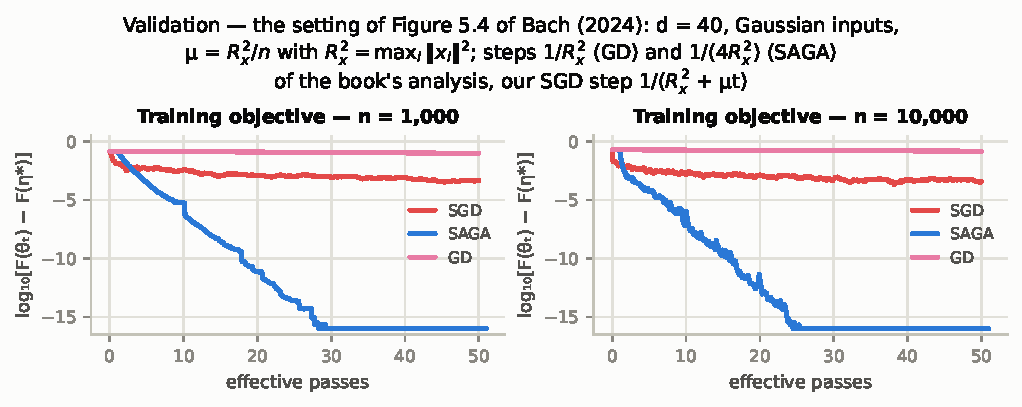
\includegraphics[width=\textwidth]{fig0_validation_book}
  \caption{\textbf{Validation on the setting of Figure~5.4 of~\cite{bach2024learning}.} $\ell_2$-regularized logistic
  regression with $d=40$ standard Gaussian features, $y=\mathrm{sign}(x^\top w+\text{noise})$, $\lambda=\mu=R_x^2/n$ with
  the book's constant $R_x^2=\max_i\norm{x_i}^2$, the steps of the book's analysis, GD $1/R_x^2$ and SAGA $1/(4R_x^2)$, and
  our SGD step $1/(R_x^2+\mu t)$. Training objective $F(\theta_t)-F(\etastar)$ against effective passes for $n=1{,}000$
  (left) and $n=10{,}000$ (right), one run each. SAGA reaches $10^{-8}$ after $13.6$ and $11.4$ passes and the floor of
  double precision ($\approx10^{-16}$) in fewer than 30 passes.}
  \label{fig:validation}
\end{figure}
